\chapter{Time Plan}
\label{ch:timeplan}

The Thesis work assumed to follow the below time plan \ref{fig:time-plan} as a standard framework. It is primarily focussed on three iterations of the UX Design process with a proper user study as a minimum with the limitation of Thesis time i.e., five months. However, with available resources will strive to perform possible UX Design cycle iterations and reach quality output with this Thesis work. \\ \\ 

Each UX Design cycle iteration is planned for one month. It comprises of four steps such as, developing prototypes, plan user study, hold user study and finally assimilating the results of that iteration. Each step is planned to execute in a week time. Next, after an iteration, again develop prototypes with improvements based on previous iteration results. Thereby, three iterations are planned as seen in Figure \ref{fig:time-plan}. \\ \\

\textbf{Milestone 1} \\

As the first milestone, by the end of May month, the first iteration of the UX Design Cycle has to be completed. \\ \\ 

\textbf{Milestone 2} \\

As the second milestone, by the end of June month, the second iteration of the UX Design Cycle has to be completed. \\ \\

\textbf{Milestone 3} \\

As the third milestone, by the end of July month, the third iteration of yhe UX Design Cycle has to be completed. \\ \\ \\

\textbf{Milestone 4} \\

As the fourth and the final milestone, by the end of September month, the Thesis documentation including presentation has to be completed. \\ \\

 
\begin{figure}[h]
	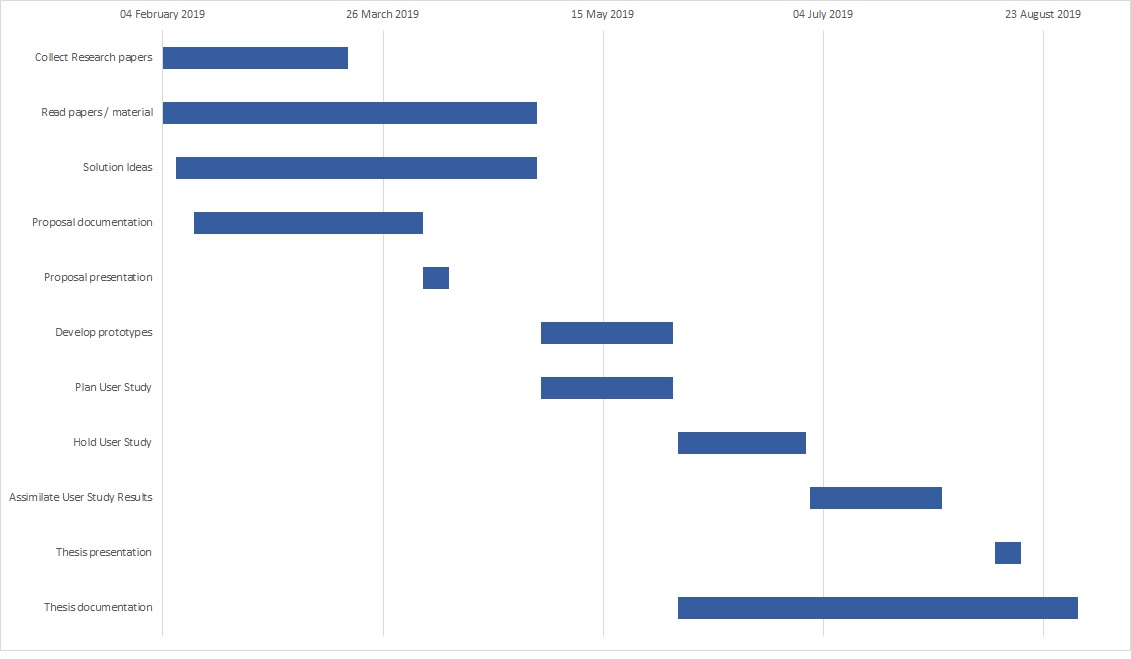
\includegraphics[width=\textwidth, frame]{Time-plan}
	\centering
	\caption{Time Plan}
	\label{fig:time-plan}
\end{figure}

